\documentclass[12pt]{article}
\usepackage{graphicx}
\usepackage[none]{hyphenat}
\usepackage{graphicx}
\usepackage{listings}
\usepackage[english]{babel}
\usepackage{graphicx}
\usepackage{caption} 
\usepackage{hyperref}
\usepackage{booktabs}
\usepackage{array}
\usepackage{amsmath}   % for having text in math mode
\usepackage{listings}
\lstset{
  frame=single,
  breaklines=true
}
  
%Following 2 lines were added to remove the blank page at the beginning
\usepackage{atbegshi}% http://ctan.org/pkg/atbegshi
\AtBeginDocument{\AtBeginShipoutNext{\AtBeginShipoutDiscard}}

%New macro definitions
\newcommand{\mydet}[1]{\ensuremath{\begin{vmatrix}#1\end{vmatrix}}}
\providecommand{\brak}[1]{\ensuremath{\left(#1\right)}}
\providecommand{\norm}[1]{\left\lVert#1\right\rVert}
\newcommand{\solution}{\noindent \textbf{Solution: }}
\newcommand{\myvec}[1]{\ensuremath{\begin{pmatrix}#1\end{pmatrix}}}
\let\vec\mathbf

\begin{document}

\begin{center}
\title{\textbf{Properties of Triangles}}
\date{\vspace{-5ex}} %Not to print date automatically
\maketitle
\end{center}
\setcounter{page}{1}

\section{10$^{th}$ Maths - Chapter 7}
This is Problem-3 from Exercise 7.1
\begin{enumerate}
\item Determine if the points $(1,5), (2,3), \text{ and } (-2,-11)$ are collinear.  \\
\solution 
 We know that points $\vec{A}, \vec{B} \text{ and } \vec{C}$ are collinear, if
\begin{align}
  \label{eq:1}
	\text{rank}\myvec{ \vec{B}-\vec{A} & \vec{C}-\vec{A}} <  2 \\
	 \vec{B}-\vec{A} &=  \myvec{
  2 \\
  3 \\
 } - \myvec{
  1 \\
  5 \\
 } &= \myvec{
 1 \\
 -2 \\
 }
 \\
\vec{C}-\vec{A} &=  \myvec{
  -2 \\
  -11 \\
 } - \myvec{
  1 \\
  5 \\
 } &= \myvec{
 -3 \\
 -16 \\
 }  \\
\label{eq:4}
\myvec{ \vec{B}-\vec{A} & \vec{C}-\vec{A}} &= \myvec{ 
       1 & -3 \\
       -2 & -16 \\
} 
\end{align}
\begin{figure}[!h]
	\begin{center}
		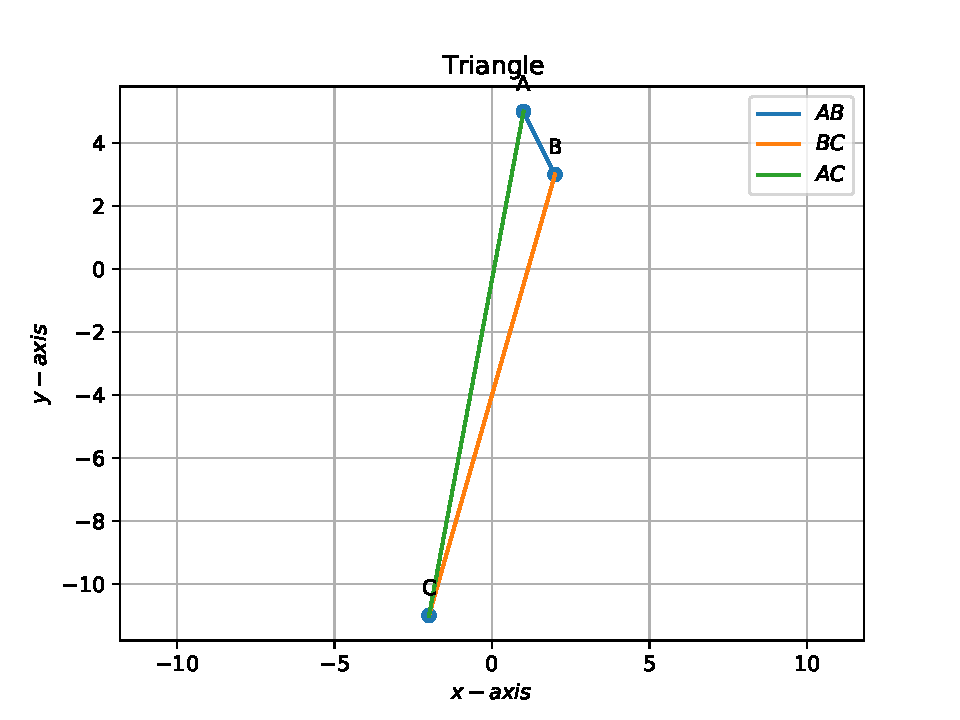
\includegraphics[width=\columnwidth]{./figs/problem3.pdf}
	\end{center}
\caption{}
\label{fig:Fig1}
\end{figure}
It is quite obvious that the above matrix mentioned in equation \ref{eq:4} has non zero determinant value implying that it is a full rank matrix with rank equal to 2. \\
Hence from equation \ref{eq:1}, it can be inferred that the points are not collinear. \\
Refer Figure \ref{fig:Fig1}.

\end{enumerate}

\end{document}
